\section{Resultat}
\label{sec:joel_a-results}
I denna del ska alla produktens miljökonsekvenser eliciteras. 

\subsection{Nivå ett effekter}
Nivå ett effekter i Greensoft modellen är de effekter som direkt följer av utvecklingen eller användningen av produkten. Den första fasen i Greensoft modellen är utvecklingsfasen och i den kan följande effekter på miljön hittas:
\begin{itemize}
	\item Strömanvändning för utvecklarnas datorer
	\item Övrig strömanvändning av utvecklarna
	\item Transport till arbetsplats
	\item Bredbandet och molntjänster utvecklarna använde sig av under utvecklingen
\end{itemize}

Projektet att skapa produkten ingick i en större universitetskurs som tog 3200 arbetstimmar för hela gruppen, uppskattningsvis kan åtminstone hälften av denna tit sägas ha lagts på produkten. Gruppen bestod av åtta personer som framförallt arbetade med produkten på sina laptops. All utvecklingstid gjordes dock inte vid en dator, visa moment såsom skapandet av arkitekturen och gruppmöten så användes ingen dator. Dessutom så skedde delar av utveckling med flera gruppmedlemmar vid samma dator. För att få in detta i uppskattningen kan vi säga att 90\% av utvecklingstiden skedde med en laptop. Så totalt blir strömanvändningen 1600 * 8 * 0.9 * x, där x står för den genomsnittliga strömanvändningen för en laptop. Eftersom en laptops strömanvändning beror på så många faktorer är det svårt att få en korrekt uppskattning av hur mycket ström som används. En ungefär värde på x kan fås genom observationen att en av medlemmarnas laptop kunde användas i ungefär fyra timmar innan den behövde laddas. Denna laptop är av modell ''Lenovo ideapad Y700'' och har enligt tillverkaren \cite{lenovo} ett batteri med 60 watt timmar. En urladdning på av detta på fyra timmar ger oss en timmes användning av 15 watt, vilket x kan approximeras till. Då får vi följande approximering för strömanvändning av datorerna gruppen använde sig av under utecklingsprocessen: $$1600 * 8 * 0.9 * 15 = 172.8kW$$

Utvecklarnas övriga strömanvändninge kommer framförallt ifrån strömanvändning i rummet där utvecklingen sker, saker såsom belysning, ventilation, och uppvärmning. Uppvärmningen av rummet kan ignoreras i detta fall då alla rum gruppen arbetade i skulle varit uppvärmda oavsett ifall de befann sig där eller inte. I stort sett all utveckling skedde i arbetsrum på Linköpings Universitet som är uppvärmda oavsett ifall de används och kontoret på Cybercom som också skulle vara uppvärmt oavsett gruppens närvaro. I energimyndighetens rapport ifrån 2007\cite{emynd} så använder det genomsnittliga svenska kontoret $23.0kWh/m^2$ för belysning och $2.6kWh/m^2$ för ventilation. En approximering av storleken på rummen gruppen arbetade i är 15 kvadratmeter, vilket ger oss en ungefärlig strömanvändning på: $$1600 * 25.6 * 15 = 614.4kW$$

De resterande nivå ett effekterna är inte nödvändigtvis försumbara, men de är svårare att bestämma konkreta siffror. Utvecklarnas transport till arbetsplatsen skedde framförallt genom gång eller cykel och är försumbar, men kategorin internetanvändning inte är det. I utvecklingen av produkten användes molntjänster såsom Githubs automatiska tester, Google drive och ett stort antal hemsidor. Användning av detta kräver både elektricitet från utvecklarnas datorer vilket syns i approximationen, men servrarna som ''hostar'' sidorna och deras strömanvändning  finns inte med i den. Strömanvändningen av alla routrar som skickar paketen till och från utvecklarna finns inte heller med i någon approximation.

\subsection{Nivå två och tre effekter}
Nivå två effekter är effekter på miljön som uppkommer tillföljd av nivå ett effekterna eller tillfölja av användning av själva produkten. Vid skrivandetsstund har inte produkten använts av kunden än, så några nivå två eller tre effekter har inte ännu uppkommit utan de är rent spekulativa. En potentiell nivå två effekt skulle kunna vara att produkten blir populär på mässor och får personer att använda sin mobil för att spela spelet. Detta är syftet med produkten, men ur ett miljömässigt perspektiv är det en negativ konsekvens eftersom det kräver både ström och bredband. På grund av produktenssnäva användningsområde och få nivå ett effekter finns det inte heller många nivå två effekter att finna. Nivå tre effekter är samhälliga förändringar som sker ur nivå två effekter. Produkten gruppen har skapat lär ha väldigt marginell påverkan på samhället i helhet, men man kan kan se den som en del av en större förändring. En förändring som kan ske ifall produkten är framgångsrik är att flera företag börjar använda sig av spel på sina mässor för att locka personer till deras presentationer. Det skulle betyda att många fler spel behöver utvecklas samt att ström och bandbredsanvändningen på mässor skulle gå upp, vilket inte är förenligt med hållbar utveckling. De andra nivå tre effekterna som produkten kan leda till är att den hjälper till att popularisera IoT, vilket är en del av dess syfte. Detta kan ses som positivt eller negativt och beror helt på hållbar utvecklingen inom den branschen är. 


\begin{figure*}[h]
	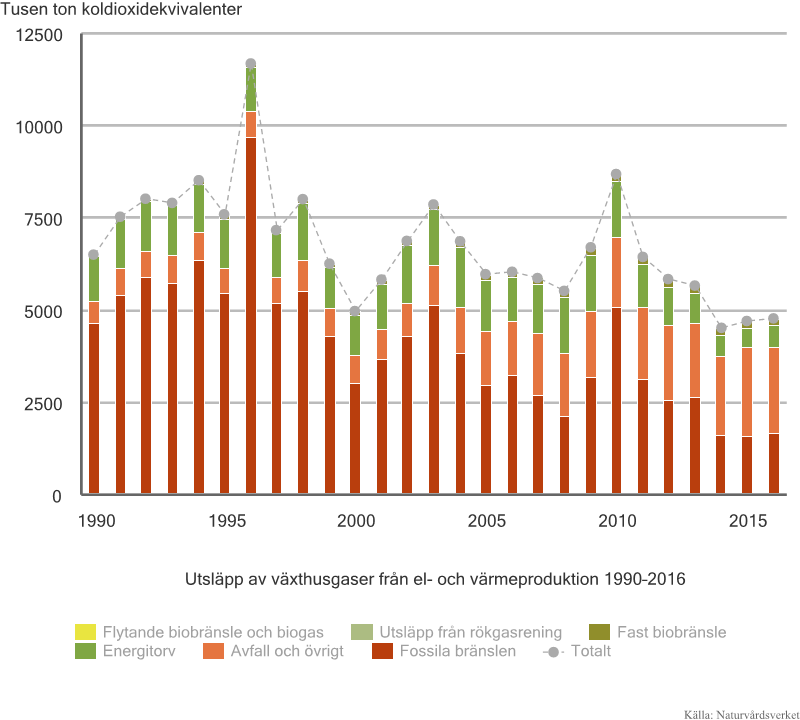
\includegraphics[scale=0.7]{naturvard-co2}
	\caption{Statistik ifrån naturvårdsverket}
	\label{natuvard-co2}
\end{figure*}


\subsection{Miljöpåverkan av utvecklingsprocessen}
Enligt \ref{natuvard-co2} så skapade Sveriges el och värmeproduktion ett CO2 utsläpp på $4781*10^9$ gram år 2016. Kombinerat med att Sveriges energi produktion detta år var 152 TWh enligt Energimyndighetens pressmeddelande\cite{elprod2016}, så får vi att varje kWh i genomsnitt skapade ett utsläpp på: $4781*10^9 / (152 * 10^{12}) \approx 31.45 * 10^{-3}$ gram CO2 per kWh. Ifrån tidigare approximerades gruppens kWh till $172.8 + 614.4 = 787.2$ vilket ger oss ett CO2 utsläpp på: $$31.45 * 10^{-3} * 787.2 \approx 24.8 \text{ gram CO2}$$
